\section*{Abstract}
\addcontentsline{toc}{section}{\protect\numberline{}Abstract}

Squats are a very common exercise used both by athletes training for sporting events, and amateurs lifting weights recreationally. As a reasonably advanced compound movement, squats can often be performed incorrectly, leading to an ineffective training program and in some cases injury. This project offers a solution to this problem, an application called \emph{Squat!}. \emph{Squat!} is a real-time squat tracking and analysis application, which uses computer vision to examine a user's squat technique whilst they are performing the lift, offering immediate feedback. In this project, a non-intrusive marker-less algorithm to track and analyse a lifter's pose using a monocular camera has been developed, and implemented to run in real-time on an Android device. The result of this project is an intuitive and accurate application for use as a training aid, enabling users to improve the safety and effectiveness of their squats.

\begin{figure}[H]
    \centering
	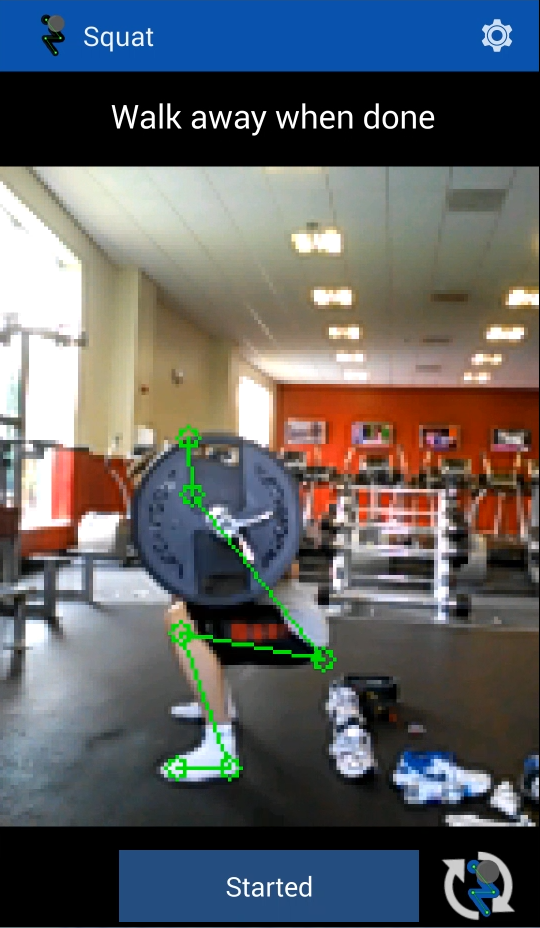
\includegraphics[height=10cm]{application/images/belowparallel}
\caption{A screenshot of the application in use}
\label{fig:preview}
\end{figure}